\documentclass{article}
\usepackage{tikz}
\usepackage{amsmath}
\begin{document}
	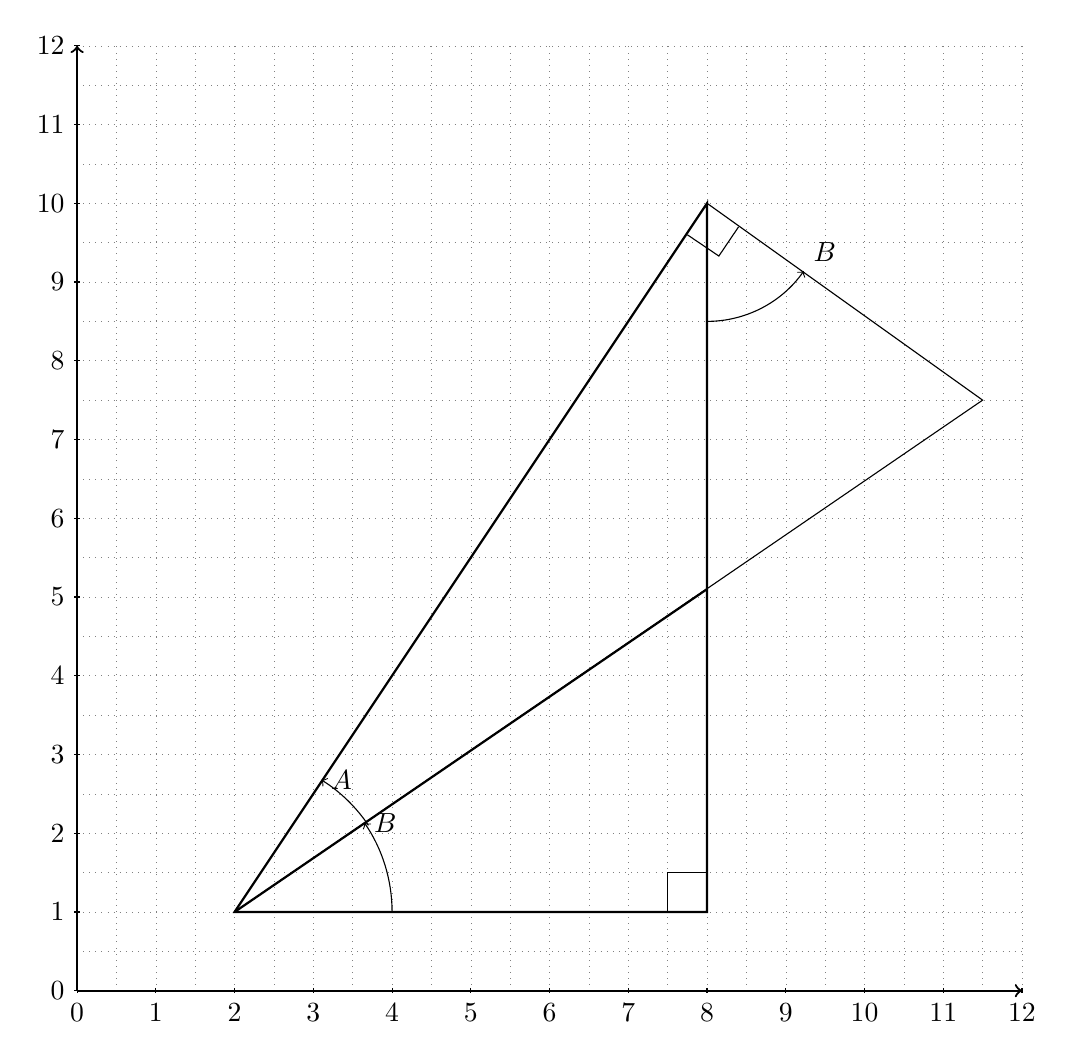
\begin{tikzpicture}
	\draw[step = 0.5 cm, gray, very thin, dotted] (0, 0) grid (12, 12);
	\draw[thick, ->] (0, 0) -- (12, 0);
	\draw[thick, ->] (0, 0) -- (0, 12);
	\foreach \x in {0, ..., 12}
	\draw (\x cm, 1 pt) -- (\x cm, -1 pt) node[anchor = north] {$\x$};
	\foreach \y in {0, ..., 12}
	\draw (1 pt, \y cm) -- (-1 pt, \y cm) node[anchor = east] {$\y$};	
	
	\draw[thick] (2, 1) -- (8, 1) -- (8, 10) -- cycle;
	\draw[thick] (2, 1) -- (8, 5.1);
	\draw[thin] (2, 1) -- (11.5, 7.5) -- (8, 10);
	
	\draw[thin, ->] (4, 1) arc (0:34.5:2) node[anchor = west] {$B$};
	\draw[thin, ->] (3.7, 2.1) arc (34:58:2) node[anchor = west] {$A$};
	\draw[thin] (7.5, 1) -- (7.5, 1.5) -- (8, 1.5);
	\draw[thin] (7.75, 9.6) -- (8.15, 9.33) -- (8.4, 9.7);
	\draw[thin, ->] (8, 8.5) arc (270:325:1.5) node[anchor = south west] {$B$};
	\end{tikzpicture}
	
	\begin{align}
	\sin{A} &= \frac{l}{h} \\
	\implies l &= h \sin{A} \\
	\cos{B} &= \frac{l}{r} \\
	\implies r &= \frac{l}{\cos{B}} \\
	&= \frac{h \sin{A}}{\cos {B}} \\
	\cos{A} &= \frac{p}{h} \\
	\implies p &= h \cos{A} \\
	\tan{B} &= \frac{t}{l} \\
	\implies t &= l \tan{B} \\
	&= h \sin{A} \tan{B} \\
	\cos{B} &= \frac{b}{q} \\
	\implies q &= \frac{b}{\cos{B}} \\
	q + t &= p \\
	\implies \frac{b}{\cos{B}} + h \sin{A} \tan{B} &= h \cos{A} \\
	\frac{b}{\cos{B}} + l \sin{A} \left(\frac{\sin{B}}{\cos{B}}\right) &= h \cos{A} \\
	b + h \sin{A} \sin{B} &= h \cos{A} \cos{B} \\
	\frac{b}{h} + \sin{A} \sin{B} &= \cos{A} \cos{B} \\
	\implies \cos \left(A + B\right) + \sin{A} \sin{B} &= \cos{A} \cos{B} \\
	\implies \cos \left(A + B\right) &= \cos{A} \cos{B} - \sin{A} \sin{B} \\
	\sin \left(A + B\right) &= \cos \left(90^{\circ} - \left(A + B\right)\right) \\ 
	&= \cos \left(\left(90^{\circ} - A\right) - B\right) \\
	&= \cos \left({90^{\circ} - A}\right) \cos \left({-B}\right) - \sin \left({90^{\circ} - A}\right) \sin \left({-B}\right) \\
	\implies \sin \left({A + B}\right) &= \sin{A} \cos{B} + \cos{A} \sin{B}
	\end{align}
\end{document}